\chapter{Cyclically fully commutative elements}

\section{Cyclically reduced elements}
    Recall that $s^{-1} = s$ for all $s \in S$, so $sws^{-1} = sws$.
    Given a word $\w = s_{x_1} s_{x_2} \cdots s_{x_k}$ for $w \in W$, a \emph{cyclic shift} of $\w$ is defined to be the natural expression that arises by conjugating $w$ by $s_{x_1}$.
    That is, $$s_{x_1} s_{x_2} \cdots s_{x_k} ~{\mapsto}~ s_{x_2} \cdots s_{x_k} s_{x_1}$$ since $s_{x_1}(s_{x_1} s_{x_2} \cdots s_{x_k})s_{x_1} = s_{x_2} \cdots s_{x_k} s_{x_1}$.

\begin{definition}\label{def:cycred}
    Let $(W,S)$ be a Coxeter system and let $\w$ be a reduced expression for some $w \in W$. If every cyclic shift of $\w$ is a reduced expression for some element in $W$, then we say that $\w$ is \emph{cyclically reduced}. A group element $w \in W$ is \emph{cyclically reduced} if every reduced expression for $w$ is cyclically reduced.
\end{definition}

    If $w$ is cyclically reduced, we can write every reduced expression for $w$ in a circle without creating any collapse in length.
    
\begin{example}\label{ex:kappa} We now consider a couple of examples.
\begin{enumerate}[label=(\alph*), leftmargin=0.75in]
\item Consider the Coxeter group of type $A_5$. Let $w \in W$ have reduced expression $\w = 31245$.
    The cyclic version of $w$ is shown in Figure~\ref{fig:circles}. In this case, $w$ is clearly cyclically reduced since there are no repeat generators. That is, we never have two adjacent occurrences of the same generator after commutations or braid moves.

\begin{center} \begin{figure}[H] \centering
\begin{tikzpicture}[scale=0.7]
    \draw[decoration={markings, mark=at position 0.05 with {\arrow{<}}},postaction={decorate}]
        (0,0) circle (2cm);
    \draw[decoration={markings, mark=at position 0.05 with {\arrow{<}}},postaction={decorate}]
        (0,0) circle (1cm);
    \draw (0,0)     node {$w$};
    \draw (90:1.5)  node {3};
    \draw (18:1.5)  node {1};
    \draw (306:1.5) node {2};
    \draw (234:1.5) node {4};
    \draw (162:1.5) node {5};
\end{tikzpicture}
\caption{Cyclically reduced group element of $W(A_4)$ written in a circle.} \label{fig:circles}
\end{figure} \end{center}

\item Consider the Coxeter group of type $A_4$. Let $w \in W$ have reduced expression $\w = 342132$. Then $w$ is not cyclically reduced, as shown in Figure~\ref{fig:notcycred}.
\begin{center} \begin{figure}[H] \centering
\begin{tabular}{m{3cm} m{0.2cm} m{3cm} m{0.2cm} m{3cm} m{0.2cm} m{3cm}}
\begin{tikzpicture}[scale=0.7]
    \draw[decoration={markings, mark=at position 0.05 with {\arrow{<}}},postaction={decorate}]
        (0,0) circle (2cm);
    \draw[decoration={markings, mark=at position 0.05 with {\arrow{<}}},postaction={decorate}]
        (0,0) circle (1cm);
    \draw (0,0)        node {$w$};
    \draw (90:1.5)     node {\textcolor{blue}{3}};
    \draw (30:1.5)     node {4};
    \draw (330:1.5)    node {2};
    \draw (270.71:1.5) node {1};
    \draw (210.28:1.5) node {\textcolor{blue}{3}};
    \draw (150.85:1.5) node {\textcolor{blue}{2}};
\end{tikzpicture} & = &
\begin{tikzpicture}[scale=0.7]
    \draw[decoration={markings, mark=at position 0.05 with {\arrow{<}}},postaction={decorate}]
        (0,0) circle (2cm);
    \draw[decoration={markings, mark=at position 0.05 with {\arrow{<}}},postaction={decorate}]
        (0,0) circle (1cm);
    \draw (0,0)        node {$w$};
    \draw (90:1.5)     node {2};
    \draw (30:1.5)     node {\textcolor{magenta}{4}};
    \draw (330:1.5)    node {\textcolor{magenta}{2}};
    \draw (270:1.5)    node {1};
    \draw (210:1.5)    node {2};
    \draw (150:1.5)    node {3};
\end{tikzpicture} & = &
\begin{tikzpicture}[scale=0.7]
    \draw[decoration={markings, mark=at position 0.05 with {\arrow{<}}},postaction={decorate}]
        (0,0) circle (2cm);
    \draw[decoration={markings, mark=at position 0.05 with {\arrow{<}}},postaction={decorate}]
        (0,0) circle (1cm);
    \draw (0,0)        node {$w$};
    \draw (90:1.5)     node {\textcolor{turq}{2}};
    \draw (30:1.5)     node {\textcolor{turq}{2}};
    \draw (330:1.5)    node {4};
    \draw (270:1.5)    node {1};
    \draw (210:1.5)    node {2};
    \draw (150:1.5)    node {3};
\end{tikzpicture} & = &
\begin{tikzpicture}[scale=0.7]
    \draw[decoration={markings, mark=at position 0.05 with {\arrow{<}}},postaction={decorate}]
        (0,0) circle (2cm);
    \draw[decoration={markings, mark=at position 0.05 with {\arrow{<}}},postaction={decorate}]
        (0,0) circle (1cm);
    \draw (0,0)        node {$w$};
    \draw (90:1.5)     node {3};
    \draw (0:1.5)      node {4};
    \draw (270.71:1.5) node {1};
    \draw (180.28:1.5) node {2};
\end{tikzpicture}
\end{tabular}
\caption{Not cyclically reduced group element of $W(A_4)$ written in a circle}\label{fig:notcycred}
\end{figure} \end{center}
\end{enumerate}
\end{example}

    Now it is natural to ask the question: Do two cyclically reduced expressions for conjugate group elements differ by a sequence of commutations, braid moves, and cyclic shifts?
    
    Unfortunately the answer is no in general, but it is often true. One of the goals of the authors of~\cite{Boothby2012} is to understand when the answer is yes.
    This motivates the following definition.

\begin{definition}\label{def:CVMT} Let $W$ be a Coxeter group. We say that a conjugacy class $C$ satisfies the \emph{cyclic version of Matsumoto's Theorem}, or CVMT, if any two cyclically reduced expressions of elements in $C$ differ by commutations, braid moves, and cyclic shifts.
\end{definition}

    We can easily find an example where the CVMT fails.

\begin{example} Let $W$ be the Coxeter group of type $A_2$. Then $1$ and $2$ (or any two distinct generators in $W(A_n)$) are conjugate since $(12)1(21) = 12121 = 21221 = 211 = 2$, but $1$ and $2$ clearly do not differ by a sequence of commutations, braid moves, and cyclic shifts.
\end{example}

    It is well known that if $s_i \in S$, then $\ell(s_i w) = \ell(w) \pm 1$, and so $\ell(w^k) \leq k \cdot \ell(w)$. If equality holds for all $k \in \N$, we say that $w$ is \emph{logarithmic}.
    If every connected component of $\Gamma_{\supp(w)}$ (that is, the subgraph of $\Gamma$ induced by the generators which appear in $w$) describes an infinite Coxeter group, then we say that $w$ is \emph{torsion-free}.

\begin{proposition}[Boothby, et al.,~\cite{Boothby2012}] \label{prop:logarithmic} Let $W$ be a Coxeter group. If $w\in W$ is logarithmic, then $w$ is cyclically reduced and torsion-free. \qed
\end{proposition}

    It follows from a result in~\cite{Speyer2009} together with the fact that Coxeter elements are trivially cyclically reduced that the converse of Proposition~\ref{prop:logarithmic} holds for Coxeter elements.

\begin{theorem}[Speyer,~\cite{Speyer2009}]\label{thm:speyer} In any Coxeter group, a Coxeter element is logarithmic if and only if it is torsion-free. \qed
\end{theorem}

    The proof of Theorem~\ref{thm:speyer} is combinatorial and relies on a natural bijection between the set $\C(W)$ of Coxeter elements and the set $\Acyc(\Gamma)$ of acyclic orientations of the Coxeter graph.
    Specifically, if $c \in \C(W)$, let $(\Gamma,c)$ denote the digraph where, if $m(s_i,s_j) \geq 3$, the edge $\{s_i,s_j\}$ in the Coxeter graph $\Gamma$ is oriented as $(s_i,s_j)$ if $s_i$ appears before $s_j$ in $c$.
    The vertex $s_{x_i}$ is a source (respectively, sink) of $(\Gamma,c)$ if and only if $s_{x_i}$ is initial (respectively, terminal) in some reduced expression for $c$. 
    Conjugating a Coxeter element $c = s_{x_1} \cdots s_{x_n}$ by $s_{x_1}$ cyclically shifts the word $s_{x_1} \cdots s_{x_n}$ to $s_{x_2} \cdots s_{x_n}s_{x_1}$ since
\begin{equation} s_{x_1}(s_{x_1}s_{x_2}\cdots s_{x_n})s_{x_1} = s_{x_2} \cdots s_{x_n}s_{x_1},\end{equation}
    and, on the level of acyclic orientations, this corresponds to converting the source vertex $s_{x_1}$ of $(\Gamma,c)$ into a sink, which takes the orientation $(\Gamma,c)$ to $(\Gamma,s_{x_1}cs_{x_1})$.
    This generates an equivalence relation $\sim_\kappa$ on $\Acyc(\Gamma)$ and on $\C(W)$.
    Two acyclic orientations $(\Gamma,c)$ and $(\Gamma,c')$ are \emph{$\kappa$-equivalent} if and only if there is a sequence $x_1,\dots,x_k$ such that $c' = s_{x_k}\cdots s_{x_1} c s_{x_1}\cdots s_{x_k}$ and $s_{x_{i+1}}$ is a source vertex of $(\Gamma,s_{x_i}\cdots s_{x_1}cs_{x_1}\cdots s_{x_i})$ for each $i=1,\dots,k-1$.
    
    Thus, two Coxeter elements $c,c' \in \C(W)$ are \emph{$\kappa$-equivalent} if they differ by a sequence of length-preserving conjugations. That is, $c \sim_\kappa c'$ if they are conjugate by $s_{x_1}\cdots s_{x_k}$ such that
    $$\ell(c) = \ell(s_{x_i} \cdots s_{x_1} c s_{x_1} \cdots s_{x_i})$$ holds for each $i = 1,\ldots, k$.

    Performing a cyclic shift of a reduced expression of an arbitrary element $w \in W$ yields an element that is conjugate to $w$, but an element conjugate to $w$ is not necessarily a cyclic shift of $w$.
    The following result by H.~Eriksson and K.~Eriksson shows that conjugation and cyclic shifts are the same for Coxeter elements.

\begin{theorem}[Eriksson--Eriksson,~\cite{Eriksson2009}] \label{thm:e2} Let $W$ be a Coxeter group and let $c, c' \in \C(W)$. Then $c$ and $c'$ are conjugate if and only if $c$ and $c'$ are $\kappa$-equivalent. \qed
\end{theorem}

\section{Cyclically fully commutative elements}\label{sec:CFC}
    Note that the Erikssons' result is the CVMT applied to Coxeter elements. Despite the fact that the CVMT does not hold in general, we wish to gain understanding about when it does.

    The proof of Theorem~\ref{thm:e2} depends on torsion-free Coxeter elements being logarithmic, and the proof of this involves combinatorial properties of the acyclic orientation construction and source-to-sink equivalence relation.
    Thus, we are motivated to extend these properties to a larger class of elements. In fact, the acyclic orientation construction above generalizes to the FC elements.
    If $w \in \FC(W)$, then $(\Gamma,w)$ is the graph whose vertices are the disjoint union of generators in any reduced expression of $w$, and a directed edge is present for each pair of noncommuting generators, with the orientation denoting which comes first in $w$.
    Since $w \in \FC(W)$, i.e., $w$ has no opportunity for braid moves, the graph $(\Gamma,w)$ is well-defined. Though the acyclic orientation construction extends from $\C(W)$ to $\FC(W)$, the source-to-sink operation does not because a cyclic shift of a reduced expression for an FC element need not be FC.
    
\begin{example} Let $w \in W(A_4)$ have reduced expression $\w = 213243$. Then $w$ is FC because there is no opportunity to apply a braid move in any reduced expression for $w$, but a cyclic shift of $\w$ is commutation equivalent to a word containing a \textcolor{blue}{blue} $\gen{23}_3$ subword since
    $$213243 \overset{2}{\mapsto} 13\textcolor{magenta}{24}32 = 134\textcolor{blue}{232}$$ after applying a commutation to the \textcolor{magenta}{pink} subword, where $\overset{i}{\longmapsto}$ indicates a cyclic shift by $i$.
\end{example}

    The previous example motivates the following definition.

\begin{definition}\label{def:CFC} An element $w \in W$ is \emph{cyclically fully commutative}, or CFC, if every cyclic shift of every reduced expression for $w$ is a reduced expression for an FC element.
\end{definition}

    We denote the set of CFC elements of $W$ by $\CFC(\Gamma)$, where $\Gamma$ is the Coxeter graph corresponding to $W$, or $\CFC(W)$.
    CFC elements are exactly the elements whose reduced expressions, when written in a circle, avoid $\gen{s,t}_{m(s,t)}$ subwords for $m(s,t) \geq 3$, and hence they are the elements for which the source-to-sink operation extends in a well-defined manner.
    The remainder of this thesis considers CFC elements.
    
\begin{example} Let $W$ be the Coxeter group of type $A_4$ and let $w, y \in W$ have reduced expressions $\w = 1243$ and $\y = 21324$, respectively. Then both $\w$ and $\y$ are FC, but, when we write each reduced expression in a circle, we have the diagrams shown in Figure~\ref{fig:circlesexample}, so $w$ is CFC because there are no opportunities for braid moves or collapses created in the circle, but $y$ is not CFC since the two adjacent occurrences of 2 collapse after commuting 2 and 4.

\begin{center} \begin{figure}[H] \centering
\begin{subfigure}{0.4\textwidth} \centering
\begin{tikzpicture}[scale=0.75]
    \draw[decoration={markings, mark=at position 0.08 with {\arrow{<}}},postaction={decorate}]
        (0,0) circle (2cm);
    \draw[decoration={markings, mark=at position 0.08 with {\arrow{<}}},postaction={decorate}]
        (0,0) circle (1cm);
    \draw (0,0)    node {$w$};
    \draw (0,1.5)  node {1};
    \draw (1.5,0)  node {2};
    \draw (0,-1.5) node {4};
    \draw (-1.5,0) node {3};
\end{tikzpicture}
\caption{}
\end{subfigure}
\begin{subfigure}{\textwidth} \centering \vspace{20pt}
\begin{tabular}{m{3cm} m{0.5cm} m{3cm} m{0.5cm} m{3cm}}
\begin{tikzpicture}[scale=0.75]
    \draw[decoration={markings, mark=at position 0.08 with {\arrow{<}}},postaction={decorate}]
        (0,0) circle (2cm);
    \draw[decoration={markings, mark=at position 0.08 with {\arrow{<}}},postaction={decorate}]
        (0,0) circle (1cm);
    \draw (0,0)     node {$y$};
    \draw (90:1.5)  node {\textcolor{magenta}{2}};
    \draw (18:1.5)  node {1};
    \draw (234:1.5) node {2};
    \draw (306:1.5) node {3};
    \draw (162:1.5) node {\textcolor{magenta}{4}};
\end{tikzpicture} & $=$ &
\begin{tikzpicture}[scale=0.75]
    \draw[decoration={markings, mark=at position 0.08 with {\arrow{<}}},postaction={decorate}]
        (0,0) circle (2cm);
    \draw[decoration={markings, mark=at position 0.08 with {\arrow{<}}},postaction={decorate}]
        (0,0) circle (1cm);
    \draw (0,0)     node {$y$};
    \draw (90:1.5)  node {4};
    \draw (18:1.5)  node {1};
    \draw (234:1.5) node {\textcolor{turq}{2}};
    \draw (306:1.5) node {3};
    \draw (162:1.5) node {\textcolor{turq}{2}};
\end{tikzpicture} & $=$ &
\begin{tikzpicture}[scale=0.75]
    \draw[decoration={markings, mark=at position 0.08 with {\arrow{<}}},postaction={decorate}]
        (0,0) circle (2cm);
    \draw[decoration={markings, mark=at position 0.08 with {\arrow{<}}},postaction={decorate}]
        (0,0) circle (1cm);
    \draw (0,0)     node {$y$};
    \draw (90:1.5)  node {4};
    \draw (330:1.5) node {1};
    \draw (210:1.5) node {3};
\end{tikzpicture} \end{tabular}
\caption{}
\end{subfigure}
\caption{Two FC elements of $W(A_4)$ written in a circle.}\label{fig:circlesexample}
\end{figure} \end{center}
\end{example}
    
\begin{remark}\label{rem:CoxCFC}
Coxeter elements are CFC since Coxeter elements are FC and any cyclic shift of a Coxeter element is still a Coxeter element.
\end{remark}
    
\begin{proposition}\label{prop:CFCsubexps} Elements corresponding to subexpressions of Coxeter elements are CFC.
\end{proposition}
\begin{proof} Let $(W,S)$ be a Coxeter system and let $w \in \C(W)$ with reduced expression $\w$. Then $w$ is FC. Let $\w'$ be a subexpression of $\w$. Generators from $S$ appear at most once in $\w'$, so $\w'$ is reduced and FC, as well.
    Hence every cyclic shift of $\w'$ has at most one appearance of each generator, so no cyclic shift of $\w'$ will have $\gen{st}_{m(s,t)}$ as a subword for all $s,t \in \supp(\w')$. Thus, the group element corresponding to $\w'$ is CFC.
\end{proof}

    The following classification of CFC elements in Coxeter groups of type $A_n$ is Proposition 5.4 in~\cite{Boothby2012}.
    
\begin{proposition}[Boothby, et al.,~\cite{Boothby2012}] \label{prop:CFCiffatmostonce} Let $w \in W(A_n)$. Then $w$ is CFC if and only if each generator in $\supp(w)$ appears exactly once. \qed
\end{proposition}

    In other words, the CFC elements in $W(A_n)$ are precisely the elements that correspond to reduced subexpressions of the Coxeter elements.

\begin{example} Let $W$ be the Coxeter group of type $A_3$. The set of CFC elements of $W$ is
	$$\CFC(A_3) = \{e, 1, 2, 3, 13, 12, 21, 23, 32, 123, 321, 132, 231\}.$$
\end{example}

\section{Cylindrical heaps}
    Let $w \in W(A_n)$ have reduced expression $\w$ and suppose $\w$ is commutation equivalent to a reduced expression that begins with $s_i$. Then a block labeled by $i$ occurs at the top of the heap $H(\w)$.
    A \emph{cyclic shift of $H(\w)$ with respect to $i$} is the heap that results from removing the block labeled by $i$ from the top of the heap and appending it to the bottom.
    In other words, if $\w$ is commutation equivalent to $s_i\u$, then a cyclic shift of $H(\w)$ with respect to $i$ is the heap $H(\u s_i)$.
    Note that $H(\u s_i)$ may not be the heap for a reduced expression. 
    However, since $\CFC(A_n) \subseteq \FC(A_n)$, any $w \in \CFC(A_n)$ has a unique heap and cyclic shifts of reduced expressions of CFC elements are reduced, so if $w$ is CFC, then $H(\u s_i)$ is the unique heap obtained by performing a cyclic shift on $w$.
    
    Consider the equivalence relation $\approx_\kappa$ generated by cyclic shifts of heaps.
    It is clear that $w$ is CFC if and only if all heaps in the equivalence class for $H(w)$ are heaps for reduced expressions of FC elements.
    Let $w, w' \in \CFC(A_n)$. Then $H(w)$ and $H(w')$ are \emph{cyclically equivalent} if $H(w)$ and $H(w')$ differ by a sequence of cyclic shifts.
    We emphasize that cyclically equivalent is only defined for heaps corresponding to CFC elements.

\begin{example} \label{ex:CFC} Let $W$ be the Coxeter group of type $A_7$.
\begin{enumerate}[leftmargin=0.75in, label=(\alph*)]
\item The group element corresponding to the heap in Figure~\ref{fig:cylheapsex1} is CFC since every sequence of cyclic shifts of the heap corresponds to a reduced expression for an FC element.
\begin{center} \begin{figure}[H] \centering \begin{tikzpicture}[scale=0.85]
    \sq{0}{2};   \node at (0.5,1.5)  {\footnotesize $4$};
    \sq{0.5}{1}; \node at (1,0.5)    {\footnotesize $5$};
    \sq{1}{0};   \node at (1.5,-0.5) {\footnotesize $6$};
    \sq{1.5}{-1};\node at (2,-1.5)   {\footnotesize $7$};
\end{tikzpicture}
\caption{The heap of a CFC element in $W(A_7)$.}\label{fig:cylheapsex1} \end{figure} \end{center}

\item The group element corresponding to the heap in Figure~\ref{fig:cylheapsex2.1} is FC because there is no opportunity to apply a braid move, but it is not CFC since the blocks labeled 2 collapse after a cyclic shift, where $\overset{2}{\mapsto}$ denotes a cyclic shift with respect to 2.

\begin{center} \begin{figure}[H] \centering
\begin{subfigure}{0.35\textwidth} \centering
\begin{tikzpicture}[scale=0.85]
    \sq{0.5}{2}; \node at (1,1.5)   {\footnotesize $2$};
    \sq{0}{1};   \node at (0.5,0.5) {\footnotesize $1$};
    \sq{1}{1};   \node at (1.5,0.5) {\footnotesize $3$};
    \sq{0.5}{0}; \node at (1,-0.5)  {\footnotesize $2$};
\end{tikzpicture} \caption{}\label{fig:cylheapsex2.1}
\end{subfigure}
\begin{subfigure}{0.55\textwidth} \centering
\begin{tabular}{m{1.75cm} m{0.75cm} m{1.75cm} m{0.75cm} m{1.75cm}}
\begin{tikzpicture}[scale=0.85]
    \sq{0.5}{2}; \node at (1,1.5)   {\footnotesize $2$};
    \sq{0}{1};   \node at (0.5,0.5) {\footnotesize $1$};
    \sq{1}{1};   \node at (1.5,0.5) {\footnotesize $3$};
    \sq{0.5}{0}; \node at (1,-0.5)  {\footnotesize $2$};
\end{tikzpicture} & $\overset{2}{\longmapsto}$ &
\begin{tikzpicture}[scale=0.85]
    \sq{0.5}{-1}; \node at (1,-1.5)  {\footnotesize $2$};
    \sq{0}{1};    \node at (0.5,0.5) {\footnotesize $1$};
    \sq{1}{1};    \node at (1.5,0.5) {\footnotesize $3$};
    \sq{0.5}{0};  \node at (1,-0.5)  {\footnotesize $2$};
\end{tikzpicture} & $\equiv$ &
\begin{tikzpicture}[scale=0.85]
    \sq{0}{1}; \node at (0.5,0.5) {\footnotesize $1$};
    \sq{1}{1}; \node at (1.5,0.5) {\footnotesize $3$};
\end{tikzpicture}
\end{tabular} \caption{}\label{fig:cylheapsex2.2}
\end{subfigure}
\caption{The heap of an FC (but not CFC) element in $W(A_7)$.}\label{fig:cylheapsex2}
\end{figure} \end{center}

\item The group element corresponding to the heap in Figure~\ref{fig:cylheapsex3} is not CFC since it is not even FC by Proposition~\ref{prop:convexsubheap}; $w$ has a reduced expression with $\gen{23}_3$ as a subword, highlighted in \textcolor{blue}{blue} in the heap.
\begin{center} \begin{figure}[H] \centering \begin{tikzpicture}[scale=0.85]
    \sqbl{0.5}{3};  \node at (1,2.5)   {\footnotesize $2$};
    \sqbl{1}{2};    \node at (1.5,1.5) {\footnotesize $3$};
    \sqbl{0.5}{1};  \node at (1,0.5)   {\footnotesize $2$};
    \sq{0}{0};      \node at (0.5,-0.5){\footnotesize $1$};
\end{tikzpicture} \caption{The heap of a non-FC element in $W(A_7)$.}\label{fig:cylheapsex3}
\end{figure} \end{center}
\end{enumerate}
\end{example}
    
    We let $\hat{H}(w)$ represent the equivalence class of CFC heaps cyclically equivalent to $H(w)$, which we visualize by wrapping representatives on a cylinder.
    We call $\hat{H}(w)$ a \emph{cylindrical heap}.

\begin{example} Let $w \in \CFC(A_4)$ have reduced expression $1324$. Then $\hat{H}(w)$ can be represented by the cylindrical heap shown in Figure~\ref{fig:cylheap1324}, where we identify the edges of the north and south faces so that the arrows match direction.
    The elements of $\hat{H}(w)$ are shown in Figure~\ref{fig:cylheapelements}.

\begin{center} \begin{figure}[H] \centering
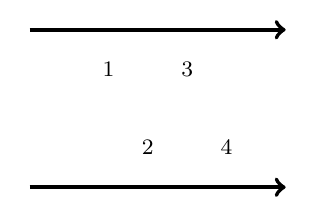
\begin{tikzpicture}
\draw[line width=1.5pt,->] (-0.5,1)--(2.75,1); \draw[line width=1.5pt,->] (-0.5,-1)--(2.75,-1);
    \sq{0}{1};   \node at (0.5,0.5) {\footnotesize $1$};
    \sq{1}{1};   \node at (1.5,0.5) {\footnotesize $3$};
    \sq{0.5}{0}; \node at (1,-0.5)  {\footnotesize $2$};
    \sq{1.5}{0}; \node at (2,-0.5)  {\footnotesize $4$};
\end{tikzpicture}
\caption{The cylindrical heap for a CFC element in $W(A_4)$.}\label{fig:cylheap1324}
\end{figure} \end{center}

\begin{center} \begin{figure}[htpb] \centering
\begin{tabular}{m{2cm} m{0.4cm} m{2cm} m{0.4cm} m{2cm} m{0.4cm} m{2cm} m{0.4cm}}
\begin{tikzpicture}[scale=0.85]
    \sq{0}{1};   \node at (0.5,0.5) {\footnotesize $1$};
    \sq{1}{1};   \node at (1.5,0.5) {\footnotesize $3$};
    \sq{0.5}{0}; \node at (1,-0.5)  {\footnotesize $2$};
    \sq{1.5}{0}; \node at (2,-0.5)  {\footnotesize $4$};
\end{tikzpicture} & , &
\begin{tikzpicture}[scale=0.85]
    \sq{0}{1};   \node at (0.5,0.5) {\footnotesize $1$};
    \sq{1}{-1};  \node at (1.5,-1.5){\footnotesize $3$};
    \sq{0.5}{0}; \node at (1,-0.5)  {\footnotesize $2$};
    \sq{1.5}{0}; \node at (2,-0.5)  {\footnotesize $4$};
\end{tikzpicture} & , &
\begin{tikzpicture}[scale=0.85]
    \sq{0}{-1};  \node at (0.5,-1.5){\footnotesize $1$};
    \sq{1}{-1};  \node at (1.5,-1.5){\footnotesize $3$};
    \sq{0.5}{0}; \node at (1,-0.5)  {\footnotesize $2$};
    \sq{1.5}{0}; \node at (2,-0.5)  {\footnotesize $4$};
\end{tikzpicture} & , &
\begin{tikzpicture}[scale=0.85]
    \sq{0}{-1};  \node at (0.5,-1.5){\footnotesize $1$};
    \sq{1}{-1};  \node at (1.5,-1.5){\footnotesize $3$};
    \sq{0.5}{0}; \node at (1,-0.5)  {\footnotesize $2$};
    \sq{1.5}{-2};\node at (2,-2.5)  {\footnotesize $4$};
\end{tikzpicture} & , \\ &&&&&&& \\
\begin{tikzpicture}[scale=0.85]
    \sq{0}{2};   \node at (0.5,1.5) {\footnotesize $1$};
    \sq{1}{0};   \node at (1.5,-0.5){\footnotesize $3$};
    \sq{0.5}{1}; \node at (1,0.5)   {\footnotesize $2$};
    \sq{1.5}{-1};\node at (2,-1.5)  {\footnotesize $4$};
\end{tikzpicture} & , &
\begin{tikzpicture}[scale=0.85]
    \sq{1.5}{3}; \node at (2,2.5)   {\footnotesize $4$};
    \sq{0}{2};   \node at (0.5,1.5) {\footnotesize $1$};
    \sq{1}{2};   \node at (1.5,1.5) {\footnotesize $3$};
    \sq{0.5}{1}; \node at (1,0.5)   {\footnotesize $2$};
\end{tikzpicture} & , &
\begin{tikzpicture}[scale=0.85]
    \sq{1}{3};   \node at (1.5,2.5) {\footnotesize $3$};
    \sq{0.5}{2}; \node at (1,1.5)   {\footnotesize $2$};
    \sq{1.5}{2}; \node at (2,1.5)   {\footnotesize $4$};
    \sq{0}{1};   \node at (0.5,0.5) {\footnotesize $1$};
\end{tikzpicture} & , &
\begin{tikzpicture}[scale=0.85]
    \sq{0}{1};   \node at (0.5,0.5) {\footnotesize $1$};
    \sq{0.5}{2}; \node at (1,1.5)   {\footnotesize $2$};
    \sq{1}{3};   \node at (1.5,2.5) {\footnotesize $3$};
    \sq{1.5}{4}; \node at (2,3.5)   {\footnotesize $4$};
\end{tikzpicture} &
\end{tabular}
\caption{The elements of the equivalence class of CFC heaps cyclically equivalent the heap of some $w \in \CFC(A_4)$.}\label{fig:cylheapelements}
\end{figure} \end{center}
\end{example}

\begin{remark}\label{rem:CFCcylinderwrap}
Even though we lose the underlying poset structure when we wrap a heap on a cylinder, a convex subheap retains its natural meaning on the cylinder.
    An element $w \in W(A_n)$ is CFC if and only if the cylindrical heap of $w$ does not contain any representatives having any convex subheaps shown in Figure~\ref{fig:convexsubheapsnotinCFC}.
    
\begin{center} \begin{figure}[htpb] \centering
\begin{subfigure}{0.25\textwidth} \centering
\begin{tikzpicture}
    \sq{0}{2};    \node at (0.5,1.5) {\scalebox{0.85}{$i$}};
    \sq{0}{1};    \node at (0.5,0.5) {\scalebox{0.85}{$i$}};
\end{tikzpicture}
\caption{}\label{}
\end{subfigure}
\begin{subfigure}{0.25\textwidth} \centering
\begin{tikzpicture}
    \sq{0}{3};    \node at (0.5,2.5) {\scalebox{0.85}{$i$}};
    \sq{0.5}{2};  \node at (1,1.5)   {\scalebox{0.85}{$i+1$}};
    \sq{0}{1};    \node at (0.5,0.5) {\scalebox{0.85}{$i$}};
    \bsq{-0.5}{2};
\end{tikzpicture}
\caption{}\label{}
\end{subfigure}
\begin{subfigure}{0.25\textwidth} \centering
\begin{tikzpicture}
    \sq{0}{3};    \node at (0.5,2.5) {\scalebox{0.85}{$i$}};
    \sq{-0.5}{2}; \node at (0,1.5)   {\scalebox{0.85}{$i-1$}};
    \sq{0}{1};    \node at (0.5,0.5) {\scalebox{0.85}{$i$}};
    \bsq{0.5}{2};
\end{tikzpicture}
\caption{}\label{}
\end{subfigure}
\caption{The convex subheaps not allowed in the heaps for CFC elements.}\label{fig:convexsubheapsnotinCFC}
\end{figure} \end{center}
\end{remark}

\begin{example}\label{ex:A4boxes} Consider the Coxeter group of type $A_4$. Recall that generators appear at most once in CFC elements, by Proposition~\ref{prop:CFCiffatmostonce}.
    The collection of boxes in Figure~\ref{fig:A4boxes} contain all reduced expressions for CFC elements in $W(A_4)$.
    The reduced expressions are grouped into boxes that contain reduced expressions for CFC elements that differ by commutations and cyclic shifts. We clearly have no opportunity for braid moves because we only consider CFC elements.
    If two reduced expressions are listed in the same column in a box, then they are reduced expressions for the same CFC element. Alternatively, a column in a particular box corresponds to a commutation class of reduced expressions.
    
    The boxes are colored based on conjugacy. That is, if two reduced expressions are in boxes of the same color (or the same box), then the corresponding CFC elements are conjugate.
    If two reduced expressions are in the same box, then the corresponding CFC elements differ by a sequence of cyclic shifts, i.e., the reduced expressions look the same, up to commutation, when written in a circle.
    
    Note that all of the CFC elements in the \textcolor{blue}{blue} box are conjugate by Theorem \ref{thm:e2} since they are Coxeter elements.
    Also, the conjugacy class for $123$ is the set of all CFC elements, i.e., columns, in the \textcolor{magenta}{pink} boxes. Its conjugacy class is partitioned into two subsets, or \emph{cyclic classes}, each of which corresponds to a cylindrical heap.
    That is, the heaps of all the reduced expressions in the box with $123$ are cyclically equivalent, and so the cylindrical heap for this box is shown in Figure~\ref{fig:cylheap123}.
    The heaps of all the reduced expressions in the box with $234$ yield the cylindrical heap shown in Figure~\ref{fig:cylheap234}.

\begin{center} \begin{figure}[H] \centering
\begin{subfigure}{0.3\textwidth} \centering
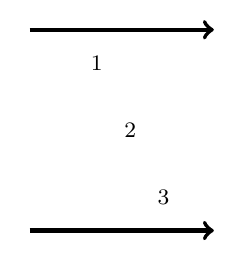
\begin{tikzpicture}[scale=0.85]
\draw[line width=1.5pt,->] (-0.5,2)--(2.25,2); \draw[line width=1.5pt,->] (-0.5,-1)--(2.25,-1);
    \sq{0}{2};   \node at (0.5,1.5)  {\footnotesize $1$};
    \sq{0.5}{1}; \node at (1,0.5)    {\footnotesize $2$};
    \sq{1}{0};   \node at (1.5,-0.5) {\footnotesize $3$};
\end{tikzpicture}
\caption{}\label{fig:cylheap123}
\end{subfigure}
\begin{subfigure}{0.3\textwidth} \centering
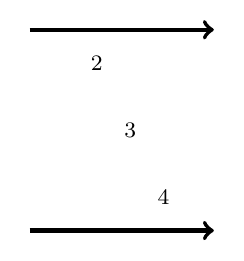
\begin{tikzpicture}[scale=0.85]
\draw[line width=1.5pt,->] (-0.5,2)--(2.25,2); \draw[line width=1.5pt,->] (-0.5,-1)--(2.25,-1);
    \sq{0}{2};   \node at (0.5,1.5)  {\footnotesize $2$};
    \sq{0.5}{1}; \node at (1,0.5)    {\footnotesize $3$};
    \sq{1}{0};   \node at (1.5,-0.5) {\footnotesize $4$};
\end{tikzpicture}
\caption{}\label{fig:cylheap234}
\end{subfigure}
\caption{The cylindrical heaps corresponding to cyclic classes of CFC elements of $W(A_4)$.}\label{fig:cylheaps123and234}
\end{figure} \end{center}
    
    We are able to move between the cyclic classes since the elements are all conjugate. It is disappointing that we cannot say everything conjugate to $123$ is conjugate by cyclic shifts (a generalization of Theorem~\ref{thm:e2}). Thus, we need another way to move between the cyclic classes.
    It turns out that we can just ``slide" the cylindrical heaps to move from the cyclic class containing $123$ to the cyclic class containing $234$. We will discuss this in more detail in Section~\ref{sec:chunks}.

\begin{center} \begin{figure}[ht!] \centering \begin{tabular}{c}
$$\boxed{~e~}$$ \\ \\
%
$\ds{\begin{array}{ccccccc}
\boxp{~1~} && \boxp{~2~} && \boxp{~3~} && \boxp{~4~}
\end{array}}$ \\ \\
%
$\ds{\begin{array}{ccccc}
\boxor{\begin{array}{c} 13 \\ 31 \end{array}} &&
\boxor{\begin{array}{c} 24 \\ 42 \end{array}} &&
\boxor{\begin{array}{c} 14 \\ 41 \end{array}}
\end{array}}$ \\ \\
%
${\ds 
\setlength{\arrayrulewidth}{1.25pt}
\begin{array}{ccccc}
\boxgr{
\begin{array}{c|c}\arrayrulecolor{ggreen}
12 & 21 \end{array}} 
&&
\boxgr{
\begin{array}{c|c}\arrayrulecolor{ggreen}
23 & 32 \end{array}}
&&
\boxgr{ 
\begin{array}{c|c}\arrayrulecolor{ggreen}
34 & 43 \end{array}}
\end{array}}$ \\ \\
%
${\ds
\setlength{\arrayrulewidth}{1.25pt}
\begin{array}{ccc}
\boxm{
\begin{array}{c|c|c|c}\arrayrulecolor{magenta}
123 & 213 & 132 & 321 \\
    & 231 & 312 &
\end{array}} 
& &
\boxm{
\begin{array}{c|c|c|c}\arrayrulecolor{magenta}
234 & 243 & 324 & 432 \\
    & 423 & 342 &
\end{array}}
\end{array}}$ \\ \\
%
${\ds
\setlength{\arrayrulewidth}{1.25pt}
\begin{array}{ccccccc}
\boxt{\begin{array}{c} 124 \\ 142 \\ 412 \end{array}} &&
\boxt{\begin{array}{c} 134 \\ 314 \\ 341 \end{array}} &&
\boxt{\begin{array}{c} 143 \\ 413 \\ 431 \end{array}} &&
\boxt{\begin{array}{c} 214 \\ 241 \\ 421 \end{array}}
\end{array}}$ \\ \\
%
$$\boxbl{
\setlength{\arrayrulewidth}{1.25pt}
\begin{array}{l|l|l|l|l|l|l|l}\arrayrulecolor{darkblue}
    1234 & 4321 & 1243 & 2134 & 3421 & 4312 & 1324 & 2143 \\
         &      & 1423 & 2314 & 3241 & 4132 & 3124 & 2413 \\
         &      & 4123 & 2341 & 3214 & 1432 & 1342 & 2431 \\
         &      &      &      &      &      & 3142 & 4213 \\
         &      &      &      &      &      & 3412 & 4231
\end{array}}$$
\end{tabular}
\caption{The conjugacy, cyclic, and commutation classes of CFC elements in $W(A_4)$.} \label{fig:A4boxes} 
\end{figure} \end{center}
\end{example}

    In~\cite{Stembridge1996}, Stembridge classified the Coxeter groups that contain finitely many FC elements (Theorem~\ref{thm:FCfinite}). Similarly, the \emph{CFC-finite groups} can be defined as the Coxeter groups that contain only finitely many CFC elements.

\begin{theorem}[Boothby, et al.,~\cite{Boothby2012}] \label{thm:CFCfinite}
    The irreducible CFC-finite Coxeter groups are $A_n$  with $n\geq 1$, $B_n$ with $n\geq 2$ , $D_n$ with $n\geq 4$, $E_n$ with $n\geq 6$, $F_n$ with $n\geq 4$, $H_n$ with $n\geq 3$, and $I_2(m)$ with $5 \leq m < \infty$. Thus, a Coxeter group is CFC-finite if and only if it is FC-finite. The graphs of FC- and CFC-finite Coxeter groups are shown in Figure~\ref{fig:coxgraphs}. \qed
\end{theorem}

\section{Pattern avoidance for CFC elements}\label{sec:Sn}
    In this section, $W$ refers to the Coxeter group of type $A_n$. Recall that $W$ is isomorphic to the symmetric group $S_{n+1}$ via the mapping that sends $s_i$ to the adjacent transposition $(i~i+1)$.
    Also recall that every permutation can be written uniquely (up to commutation) as a product of disjoint cycles.
    We will not make a distinction between an element from $W(A_n)$ and the corresponding permutation in $S_{n+1}$.

    As a convention, we will multiply (compose) permutations right to left.
    Recall that if $w \in S_n$, then $[w(1)~w(2) \cdots w(n)]$ is the \emph{one-line notation} corresponding to $w$. Note the use of brackets.

\begin{example} Let $W$ be the Coxeter graph of type $A_4$. Let $w \in W$ have reduced expression $\w = 12342$.
    Then the corresponding permutation in $S_5$ is $$(12)(23)(34)(45)(23) = (1245).$$
    Then, in one-line notation, we have $$(1245) = [24351]$$ since 1 is sent to 2, 2 is sent to 4, 3 is sent to itself, 4 is sent to 5, and 5 is sent back to 1.
\end{example}

    We can depict the one-line notation of a permutation $w$ as a graph to see its shape. A \emph{permutation line graph} has line segments joining $(i,w(i))$ to $(i+1,w(i+1))$ for each $1 \leq i \leq n-1$.

\begin{example}\label{ex:linegraphs} We consider some permutation line graphs.
\begin{enumerate}[label=(\alph*),leftmargin=0.75in]
\item Consider the permutation $w = [2413]$. Then the permutation line graph is shown in Figure~\ref{fig:permlinegraphs1}.

\item Consider the permutation $w = [315462]$. Then the permutation line graph is shown in Figure~\ref{fig:permlinegraphs2}.
\end{enumerate}

\begin{center} \begin{figure}[ht!] \centering
\begin{subfigure}{0.4\textwidth} \centering \vspace{35pt}
\begin{tikzpicture}[scale=0.95] \begin{scriptsize}
\draw (0,0)--(4.5,0); \draw (0,0)--(0,4.5);
\foreach \x in {1,2,3,4} \draw[shift={(\x,0)},color=black] (0pt,2pt)--(0pt,-2pt);
\foreach \y in {1,2,3,4} \draw[shift={(0,\y)},color=black] (2pt,0pt)--(-2pt,0pt);
    \draw (1,-0.25) node {$1$};
    \draw (2,-0.25) node {$2$};
    \draw (3,-0.25) node {$3$};
    \draw (4,-0.25) node {$4$};
    \draw (-0.25,1)  node {$1$};
    \draw (-0.25,2)  node {$2$};
    \draw (-0.25,3)  node {$3$};
    \draw (-0.25,4)  node {$4$};
    \draw[fill=black] (1,2) circle (1pt);
    \draw[fill=black] (2,4) circle (1pt);
    \draw[fill=black] (3,1) circle (1pt);
    \draw[fill=black] (4,3) circle (1pt);
    \draw (1,2)--(2,4)--(3,1)--(4,3);
\end{scriptsize} \end{tikzpicture}
\caption{}
\label{fig:permlinegraphs1}
\end{subfigure}
\begin{subfigure}{0.4\textwidth} \centering
\begin{tikzpicture}[scale=0.85] \begin{scriptsize}
\draw (0,0)--(6.5,0); \draw (0,0)--(0,6.5);
\foreach \x in {1,2,3,4,5,6} \draw[shift={(\x,0)},color=black] (0pt,2pt)--(0pt,-2pt);
\foreach \y in {1,2,3,4,5,6} \draw[shift={(0,\y)},color=black] (2pt,0pt)--(-2pt,0pt);
    \draw (1,-0.25) node {$1$};
    \draw (2,-0.25) node {$2$};
    \draw (3,-0.25) node {$3$};
    \draw (4,-0.25) node {$4$};
    \draw (5,-0.25) node {$5$};
    \draw (6,-0.25) node {$6$};
    \draw (-0.25,1) node {$1$};
    \draw (-0.25,2) node {$2$};
    \draw (-0.25,3) node {$3$};
    \draw (-0.25,4) node {$4$};
    \draw (-0.25,5) node {$5$};
    \draw (-0.25,6) node {$6$};
    \draw[fill=black]   (1,3) circle (1pt);
    \draw[fill=black]   (2,1) circle (1pt);
    \draw[fill=black]   (3,5) circle (1pt);
    \draw[fill=black]   (4,4) circle (1pt);
    \draw[fill=black]   (5,6) circle (1pt);
    \draw[fill=black]   (6,2) circle (1pt);
    \draw (1,3)--(2,1)--(3,5)--(4,4)--(5,6)--(6,2);
\end{scriptsize} \end{tikzpicture}
\caption{}
\label{fig:permlinegraphs2}
\end{subfigure}
\caption{Permutation line graphs.}\label{fig:permlinegraphsexample}
\end{figure}
\end{center}
\end{example}

    Using the notion of \emph{pattern avoidance}, we can determine whether a permutation is FC or CFC by inspecting its one-line notation.
    If $w \in W(A_n)$, then $w$ avoids the pattern $321$ if there is no subset $\{i,j,k\} \subseteq \{1,\ldots,n+1\}$ with $i < j < k$ and $w(k) < w(j) < w(i)$.
    Similarly, a permutation $w$ avoids the pattern $3412$ if there is no subset $\{i,j,k,\ell\} \subseteq \{1,\ldots,n+1\}$ with $i < j < k < \ell$ and $w(k) < w(\ell) < w(i) < w(j)$.
    
    Note that the elements that constitute the 321 and 3412 patterns need not be consecutive. To have a 321 pattern, the one-line notation must have a strictly descending subsequence of three elements.
    Portions of the permutation line graphs corresponding to the patterns 321 and 3412 are shown in Figure~\ref{fig:patternmountains}.

\begin{center} \begin{figure}[h!]
\begin{subfigure}{3in} \centering \vspace{10pt}
\begin{tikzpicture}
\draw (0,0)--(3.5,0); \draw (0,0)--(0,3.5);
\foreach \x in {1,2,3} \draw[shift={(\x,0)},color=black] (0pt,2pt)--(0pt,-2pt);
\foreach \y in {1,2,3} \draw[shift={(0,\y)},color=black] (2pt,0pt)--(-2pt,0pt);
\begin{scriptsize}
    \draw (1,-0.3) node {$i$};
    \draw (2,-0.3) node {$j$};
    \draw (3,-0.3) node {$k$};
    \draw (-0.4,1) node {$w(k)$};
    \draw (-0.4,2) node {$w(j)$};
    \draw (-0.4,3) node {$w(i)$};
    \draw[fill=black] (1,3) circle (1.5pt);
    \draw[fill=black] (2,2) circle (1.5pt);
    \draw[fill=black] (3,1) circle (1.5pt);
    \draw (0.5,-0.3) node {$\cdots$};
    \draw (1.5,-0.3) node {$\cdots$};
    \draw (2.5,-0.3) node {$\cdots$};
    \draw (-0.4,0.5) node {$\vdots$};
    \draw (-0.4,1.55) node {$\vdots$};
    \draw (-0.4,2.55) node {$\vdots$};
\end{scriptsize}\end{tikzpicture}
\caption{The pattern 321}\label{fig:321}
\end{subfigure}
\begin{subfigure}{3in} \centering
\begin{tikzpicture}[scale=0.85]
\draw (0,0)--(4.5,0); \draw (0,0)--(0,4.5);
\foreach \x in {1,2,3,4} \draw[shift={(\x,0)},color=black] (0pt,2pt)--(0pt,-2pt);
\foreach \y in {1,2,3,4} \draw[shift={(0,\y)},color=black] (2pt,0pt)--(-2pt,0pt);
\begin{scriptsize}
    \draw (1,-0.3) node {$i$};
    \draw (2,-0.3) node {$j$};
    \draw (3,-0.3) node {$k$};
    \draw (4,-0.3) node {$\ell$};
    \draw (-0.5,1) node {$w(k)$};
    \draw (-0.5,2) node {$w(\ell)$};
    \draw (-0.5,3) node {$w(i)$};
    \draw (-0.5,4) node {$w(j)$};
    \draw[fill=black] (1,3) circle (2pt);
    \draw[fill=black] (2,4) circle (2pt);
    \draw[fill=black] (3,1) circle (2pt);
    \draw[fill=black] (4,2) circle (2pt);
    \draw (0.5,-0.3) node {$\cdots$};
    \draw (1.5,-0.3) node {$\cdots$};
    \draw (2.5,-0.3) node {$\cdots$};
    \draw (3.5,-0.3) node {$\cdots$};
    \draw (-0.5,0.5) node {$\vdots$};
    \draw (-0.5,1.55) node {$\vdots$};
    \draw (-0.5,2.55) node {$\vdots$};
    \draw (-0.5,3.55) node {$\vdots$};
\end{scriptsize} \end{tikzpicture}
\caption{The pattern 3412}\label{fig:3412}
\end{subfigure}
\caption{The permutation line graphs of the 321 and 3412 patterns.} \label{fig:patternmountains}
\end{figure} \end{center}

\begin{example}\label{ex:patterns} Let $w \in W(A_5)$ have reduced expression $\w = 234513$. Then $w$ corresponds to $$(23)(34)(45)(56)(12)(34) = (13562)$$ in $S_6$. The one-line notation for $w$ is $[31\textcolor{ggreen}{54}6\textcolor{ggreen}{2}]$. 
    There is a 321 pattern in the one-line notation, highlighted in \textcolor{ggreen}{green}, but there is no 3412 pattern. The permutation line graph for $[315462]$ is shown in Figure~\ref{fig:permlinegraphs2}.
\end{example}

\begin{proposition}[Billey,~\cite{Billey2007}]\label{prop:321FC} An element $w \in W(A_n)$ is FC if and only if $w$ is 321-avoiding. \qed
\end{proposition}

    As a consequence of Proposition~\ref{prop:321FC}, the element from Example~\ref{ex:patterns} is not FC.
    
    The following proposition about pattern avoidance is from~\cite{Boothby2012}.
    
\begin{proposition}[Boothby, et al.,~\cite{Boothby2012}]\label{prop:patterns} An element $w \in W(A_n)$ is CFC if and only if $w$ is $321$- and $3412$-avoiding. \qed
\end{proposition}

\begin{example}\label{ex:permscyclic} We will now explore a few examples. \begin{enumerate}[leftmargin=0.75in, label=(\alph*)]
\item Let $W$ be the Coxeter group of type $A_3$. Then $W \cong S_4$. Let $w \in W$ have reduced expression $\w = 132$. Then $w$ is CFC since $w$ is a Coxeter element. In this case, its heap is shown in Figure~\ref{fig:cycheapex1}

\begin{center} \begin{figure}[H] \centering
\begin{tikzpicture}
    \sq{0}{1};   \node at (0.5,0.5) {$1$};
    \sq{1}{1};   \node at (1.5,0.5) {$3$};
    \sq{0.5}{0}; \node at (1,-0.5)  {$2$};
\end{tikzpicture}
\caption{The heap for a CFC element in $W(A_3)$.}\label{fig:cycheapex1}
\end{figure} \end{center}
    We see that $w$ corresponds to the permutation $(12)(34)(23) = (1243) = [2413]$ in $S_4$ in cycle notation and one-line notation.
    The permutation line graph is shown in part (a) of Example~\ref{ex:linegraphs}.
    Since there are only four elements and is not $[3412]$ exactly, $w$ is clearly 3412-avoiding. It is also 321-avoiding because there is not a strictly decreasing subsequence of three elements in the one-line notation. We can also see this in the permutation line graph.
    These conclusions agree with Proposition~\ref{prop:patterns}.
	
\item Let $W$ be the Coxeter group of type $A_3$. Then $W \cong S_4$. Let $w \in W$ have reduced expression $\w = 3213$. Then, in cycle and one-line notations, we have that $w$ corresponds to $$(34)(23)(12)(34) = (124) = [2431]$$ in $S_4$.
    Since $431$ in the one-line notation is a 321 pattern, $[2431]$ is not 321-avoiding.
    We can see this in the permutation line graph, shown in Figure~\ref{fig:permline2431}, where the circled points correspond to the elements that constitute the 321 pattern.
    Then, by Proposition~\ref{prop:321FC}, $w$ is not FC, and hence not CFC. In this case, the heaps for $w$ are shown in Figures~\ref{fig:heapfor3213} and~\ref{fig:heapfor2321}.
    It is clear from the heaps that $w$ is not FC because each heap contains a convex subheap corresponding to the braid relation $323 = 232$.

\begin{center} \begin{figure}[H] \centering
\begin{subfigure}{0.35\textwidth} \centering
\begin{tikzpicture}[scale=0.9]
\begin{scriptsize}
\draw (0,0)--(4.5,0); \draw (0,0)--(0,4.5);
\foreach \x in {1,2,3,4} \draw[shift={(\x,0)},color=black] (0pt,2pt)--(0pt,-2pt);
\foreach \y in {1,2,3,4} \draw[shift={(0,\y)},color=black] (2pt,0pt)--(-2pt,0pt);
    \draw (1,-0.25) node {$1$};
    \draw (2,-0.25) node {$2$};
    \draw (3,-0.25) node {$3$};
    \draw (4,-0.25) node {$4$};
    \draw (-0.8,1)  node {$1$};
    \draw (-0.8,2)  node {$2$};
    \draw (-0.8,3)  node {$3$};
    \draw (-0.8,4)  node {$4$};
    \draw[fill=black] (1,2) circle (1pt);
    \draw[fill=black] (2,4) circle (1pt); \draw[color=ggreen,line width=1pt] (2,4) circle (4pt);
    \draw[fill=black] (3,3) circle (1pt); \draw[color=ggreen,line width=1pt] (3,3) circle (4pt);
    \draw[fill=black] (4,1) circle (1pt); \draw[color=ggreen,line width=1pt] (4,1) circle (4pt);
    \draw (1,2)--(2,4)--(3,3)--(4,1);
\end{scriptsize} \end{tikzpicture}
\caption{}\label{fig:permline2431}
\end{subfigure}
\begin{subfigure}{0.225\textwidth} \centering \vspace{54pt}
\begin{tikzpicture}[scale=0.85]
    \sq{1}{2};   \node at (1.5,1.5) {$3$};
    \sq{0.5}{1}; \node at (1,0.5)   {$2$};
    \sq{0}{0};   \node at (0.5,-0.5){$1$};
    \sq{1}{0};   \node at (1.5,-0.5){$3$};
\end{tikzpicture}
\caption{}\label{fig:heapfor3213}
\end{subfigure}
\begin{subfigure}{0.225\textwidth} \centering \vspace{30pt}
\begin{tikzpicture}[scale=0.85]
    \sq{0.5}{3}; \node at (1,2.5)   {$2$};
    \sq{1}{2};   \node at (1.5,1.5) {$3$};
    \sq{0.5}{1}; \node at (1,0.5)   {$2$};
    \sq{0}{0};   \node at (0.5,-0.5){$1$};
\end{tikzpicture}
\caption{}\label{fig:heapfor2321}
\end{subfigure}
\caption{The permutation line graph and two heaps corresponding to some $w\in W(A_4)$.}\label{}
\end{figure} \end{center}


\item Let $W$ be the Coxeter group of type $A_n$ where $n$ is at least 7. Let $w \in W$ correspond to the element $[\cdots \textcolor{magenta}{5}1\textcolor{magenta}{83}2\textcolor{magenta}{4} \cdots]$ of $S_{n+1}$.
    Note that this element is not 3412-avoiding because the pink elements create a 3412 pattern. So, $w$ is not CFC.
    Moreover, $w$ is not even FC by Proposition~\ref{prop:321FC} because 832 exhibits a 321 pattern.
	
\item Let $W$ be the Coxeter group of type $A_3$. Then $W \cong S_4$. Let $w \in W$ have reduced expression $\w = 2132$. Then $w$ is FC and the heap of $w$ is shown in Figure~\ref{fig:heap2132}. Inspecting the heap makes it clear that $w$ is not CFC. Moreover, we see that the corresponding permutation is $$(23)(12)(34)(23) = (13)(24) = [3412],$$ which is obviously not 3412-avoiding but is 321-avoiding.

\begin{center} \begin{figure}[H] \centering
\begin{tikzpicture}[scale=0.85]
    \sq{0.5}{1}; \node at (1,0.5)   {$2$};
    \sq{0}{0};   \node at (0.5,-0.5){$1$};
    \sq{1}{0};   \node at (1.5,-0.5){$3$};
    \sq{0.5}{-1};\node at (1,-1.5)  {$2$};
\end{tikzpicture}
\caption{The heap of an FC element of $W(A_3)$.}\label{fig:heap2132}
\end{figure} \end{center}

\item \label{ex:cyclicshifts} Let $w \in W(A_4)$ have reduced expression $\w = 1234$. Then $w$ is FC and the heap of $w$ is shown in Figure~\ref{fig:heap1234}. Then $w$ corresponds to $(12)(23)(34)(45) = (12345)$.
    All possible sequences of cyclic shifts of $H(w)$ and their corresponding permutations in $S_5$ are shown in Figure~\ref{fig:cyclicshiftsof1234}. We shift the \textcolor{magenta}{pink} blocks to obtain the heap that follows. Since $w$ is a Coxeter element, it is CFC, and every cyclic shift of $w$ is also CFC by Remark~\ref{rem:CoxCFC}.
\begin{center} \begin{figure}[H] \centering
\begin{tikzpicture}[scale=0.85]
    \sq{0}{2};    \node at (0.5,1.5)  {\footnotesize $1$};
    \sq{0.5}{1};  \node at (1,0.5)    {\footnotesize $2$};
    \sq{1}{0};    \node at (1.5,-0.5) {\footnotesize $3$};
    \sq{1.5}{-1}; \node at (2,-1.5)   {\footnotesize $4$};
\end{tikzpicture} \caption{The heap of a CFC element of $W(A_4)$.}\label{fig:heap1234}
\end{figure} \end{center}
\end{enumerate}
\end{example}

\begin{center} \begin{figure}[h!] \centering
\begin{tabular}{@{}m{2.7cm} @{}m{0.9cm} @{}m{2.3cm} @{}m{2.7cm} @{}m{0.9cm} @{}m{1cm}}
\begin{tikzpicture}[scale=0.85]
    \sq{0}{0};    \node at (0.5,-0.5) {\footnotesize $1$};
    \sqm{0.5}{1}; \node at (1,0.5)    {\footnotesize $2$};
    \sq{1}{0};    \node at (1.5,-0.5) {\footnotesize $3$};
    \sq{1.5}{-1}; \node at (2,-1.5)   {\footnotesize $4$};
\end{tikzpicture} & $\mapsto$ &
    $(13452)$ &
\begin{tikzpicture}[scale=0.85]
    \sq{0}{0};    \node at (0.5,-0.5) {\footnotesize $1$};
    \sq{0.5}{-1}; \node at (1,-1.5)   {\footnotesize $2$};
    \sqm{1}{0};   \node at (1.5,-0.5) {\footnotesize $3$};
    \sq{1.5}{-1}; \node at (2,-1.5)   {\footnotesize $4$};
\end{tikzpicture} & $\mapsto$ &
    $(12453)$ \\ && \\
\begin{tikzpicture}[scale=0.85]
    \sqm{0}{0};   \node at (0.5,-0.5) {\footnotesize $1$};
    \sq{0.5}{-1}; \node at (1,-1.5)   {\footnotesize $2$};
    \sq{1}{-2};   \node at (1.5,-2.5) {\footnotesize $3$};
    \sq{1.5}{-1}; \node at (2,-1.5)   {\footnotesize $4$};
\end{tikzpicture} & $\mapsto$ &
    $(12354)$ &
\begin{tikzpicture}[scale=0.85]
    \sq{0}{0};    \node at (0.5,-0.5) {\footnotesize $1$};
    \sqm{0.5}{1}; \node at (1,0.5)    {\footnotesize $2$};
    \sq{1}{0};    \node at (1.5,-0.5) {\footnotesize $3$};
    \sq{1.5}{1};  \node at (2,0.5)    {\footnotesize $4$};
\end{tikzpicture} & $\mapsto$ &
    $(13542)$ \\ && \\
\begin{tikzpicture}[scale=0.85]
    \sqm{0}{0};   \node at (0.5,-0.5) {\footnotesize $1$};
    \sq{0.5}{-1}; \node at (1,-1.5)   {\footnotesize $2$};
    \sq{1}{0};    \node at (1.5,-0.5) {\footnotesize $3$};
    \sq{1.5}{1};  \node at (2,0.5)    {\footnotesize $4$};
\end{tikzpicture} & $\mapsto$ &
    $(14532)$ &
\begin{tikzpicture}[scale=0.85]
    \sq{0}{-2};   \node at (0.5,-2.5) {\footnotesize $1$};
    \sq{0.5}{-1}; \node at (1,-1.5)   {\footnotesize $2$};
    \sq{1}{0};    \node at (1.5,-0.5) {\footnotesize $3$};
    \sqm{1.5}{1}; \node at (2,0.5)    {\footnotesize $4$};
\end{tikzpicture} & $\mapsto$ &
    $(15432)$
\end{tabular}
\begin{center} \begin{tabular}{@{}m{2.7cm} @{}m{0.9cm} @{}m{1.5cm}} \vspace{14pt} \begin{tikzpicture}[scale=0.85]
    \sq{0}{0};    \node at (0.5,-0.5) {\footnotesize $1$};
    \sq{0.5}{1};  \node at (1,0.5)    {\footnotesize $2$};
    \sq{1}{2};    \node at (1.5,1.5)  {\footnotesize $3$};
    \sq{1.5}{1};  \node at (2,0.5)    {\footnotesize $4$};
\end{tikzpicture} & $\mapsto$ &
    $(14532)$
\end{tabular} \end{center}
\caption{Cyclic shifts of the heap of a CFC element of $W(A_4)$ and the corresponding permutations.}\label{fig:cyclicshiftsof1234}
\end{figure} \end{center} 


    Recall that two permutations are conjugate if and only if they have the same cycle type.
    Since Coxeter elements in $W(A_n)$ correspond to $(n+1)$-cycles in $S_{n+1}$, all Coxeter elements are conjugate as they have the same cycle type. So, all Coxeter elements are cyclically equivalent by Theorem~\ref{thm:e2} and as seen in Figure~\ref{fig:A4boxes}, but not all $(n+1)$-cycles correspond to Coxeter elements.
     
    For example, $1234 = (12)(23)(34)(45) = (12345)$. There are seven other Coxeter elements conjugate to $1234$, as shown in Figure~\ref{fig:coxeltsinA4}, but there are 24 distinct 5-cycles in $S_5$.

    Given a product of disjoint cycles, we want to be able to determine if the group element corresponding to the permutation is a CFC element.
    For example, which 4-cycles in $S_4$ correspond to CFC elements in $A_3$?
    In order to attempt to answer this question, we need a couple definitions.

    Let $(\cdots i~w(i)~w^2(i) \cdots)$ be a cycle in the permutation corresponding to $w \in W(A_n)$, assuming the smallest element appearing in the cycle is written first. Then there is a \emph{direction change at $w(i)$} if
\begin{enumerate}[label=(\alph*),leftmargin=0.75in]
    \item $i < w(i)$ and $w(i) > w^2(i)$ or
    \item $i > w(i)$ and $w(i) < w^2(i)$.
\end{enumerate}

\begin{example} Consider the symmetric group $S_6$. Let $w = (12435)$ and $y = (135)(246)$ in $S_6$. Then neither cycle for $y$ has a direction change, but there is a direction change at 4 in $w$ since $i = 2 < w(i) = 4$ and $4 = w(i) > w^2(i) = 3$. There is also a direction change at 3 in $w$.
\end{example}

    We define the \emph{support of a cycle $c$ of $w$} to be the set of numbers appearing in the cycle, denoted by $\cyclesupp(c)$.
    Note that $\cyclesupp(c)$ is not the same set as $\supp(w)$, even in the case when $w$ corresponds to a single cycle.
    We say a cycle $c$ has \emph{connected support} if the support of $c$ is a set of consecutive numbers.

\begin{example} The support of the permutation $(1357)$ is $\{1,3,5,7\}$, so $(1357)$ does not have connected support. However, the permutation $(234)$ does have connected support, namely $\cyclesupp((234)) = \{2,3,4\}$.
\end{example}

    Utilizing Sage~\cite{sage}, we witnessed evidence of the following conjecture, which we believe is true in general.

\begin{conjecture}\label{conjecture}
Let $w \in W(A_n)$ correspond to a permutation with disjoint cycles $c_1, c_2, \ldots, c_k$ in $S_{n+1}$. Assume each $c_j$ is written with the smallest number first.
    Then $w \in \CFC(A_n)$ if and only if each $c_j$ has connected support and has at most one direction change.
\end{conjecture}

\begin{example} We return to part (e) of Example~\ref{ex:permscyclic}. In that example, we have a 5-cycle corresponding to each cyclic shift of the heap of $1234$.
    Note that each of the 5-cycles satisfies both conditions of Conjecture~\ref{conjecture}.
    However, the cycle $w = (14352)$ has three direction changes, namely, at 4, 3, and 5. 
    One heap of $w$ corresponding to the reduced expression $324134$ is shown in Figure~\ref{fig:dirchangeheap}. Then $w$ is not CFC since $w$ is not FC, due to the appearance of a 434 subword, satisfying Conjecture~\ref{conjecture}.
\begin{center} \begin{figure}[H] \centering
\begin{tikzpicture}
    \sq{1}{4};   \node at (1.5,3.5) {\footnotesize $3$};
    \sq{0.5}{3}; \node at (1,2.5)   {\footnotesize $2$};
    \sq{1.5}{3}; \node at (2,2.5)   {\footnotesize $4$};
    \sq{0}{2};   \node at (0.5,1.5) {\footnotesize $1$};
    \sq{1}{2};   \node at (1.5,1.5) {\footnotesize $3$};
    \sq{1.5}{1}; \node at (2,0.5)   {\footnotesize $4$};
\end{tikzpicture}
\caption{A heap for an element of $W(A_4)$ that corresponds to a permutation in $S_5$ with more than one direction change.}\label{fig:dirchangeheap}
\end{figure} \end{center}
\end{example}
    
    Cycle type provides insight into the structure of the sets of conjugate CFC elements. However, our ultimate goal is to generalize to other types of Coxeter groups, where cycle type is not available.

